******Outline for HERA Summary********

\subsection{Software Benchmarking}

In order to establish the validity of future background simulations using current software tools, a benchmarking study was conducted using background rates and parameters from the HERA-II upgrade.  Conditions observed at HERA were replicated and rates compared to those seen in the scintillator time-of-flight detector near the IP.  Successfully reproducing these rates by simulating HERA conditions validates the software tools to be used for future background studies. 

\subsection{issues at hera and lessons learned}
Following the HERA-II upgrade in 2000/2001, significant levels of beam-induced background were observed and identified: synchrotron radiation, proton gas scattering, lepton gas scattering, and proton beam halo losses.   In fact, 95\% of background observed following the upgrade came from proton beam-gas interactions where vacuum conditions had deteriorated due to synchrotron radiation.  The background significantly impacted the detectors and initiated a several month shutdown to perform simulations and remediate the problem.

%Discuss HERA design elements which made problem worse.
%Several design choices exacerbated the background generated around the IP.  For instance, the electron and proton beams shared the same pipe, which [...].  

Rectifying the beam-gas background at HERA required dynamic pressure profile simulations, measurements of the beam pipe's pressure distribution, and residual beam gas analysis.  Results indicated that vacuum pressure increased to $10^{-8}$ mbar in the region spanning $\pm$ 5 m around the IP.   This  was 100 times higher than the nominal pressure of $10^{-10}$ mbar achieved at the location of the vacuum pumps. Analysis showed that hydrogen dominated the beam gas composition. 



\begin{figure}
	\centering
	\begin{minipage}{0.45\textwidth}
		\centering
		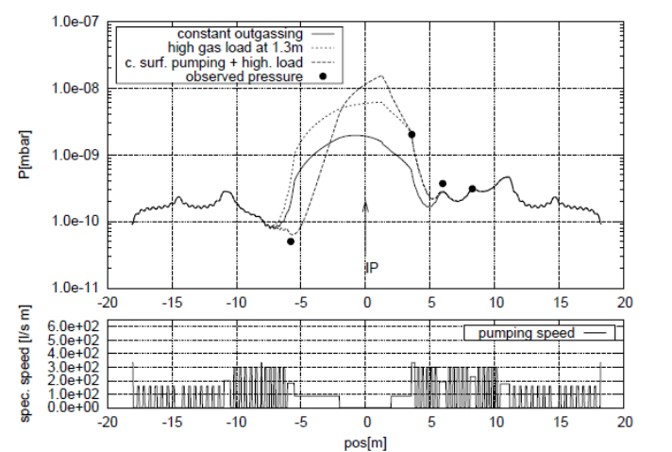
\includegraphics[width=.75\textwidth]{../../img/hera_badvac_regions.jpg}
		\caption {Left: HERA-II Vacuum pressure distribution in the IR.  }
		
	\end{minipage}\hfill
	\begin{minipage}{0.45\textwidth}
		\centering	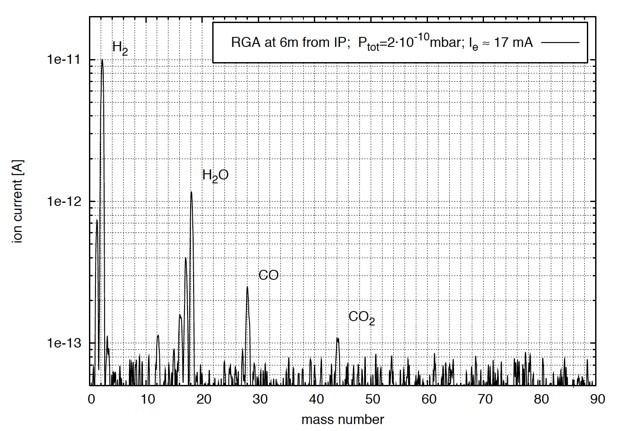
\includegraphics[width=.75\textwidth]{../../img/hera_badvac_comp.jpg}	
		\caption {HERA-II Composition of beampipe gas $\pm$ 5m around the IP. }
	\end{minipage}
	
\end{figure}


\subsection{hera configuration and rates in C5 detector-- primary images}
In particular, the C5 dual layer scintillator detector located upstream of the interaction point served as an indicator of beam-gas background as a function of current.   Although the rates in the C5 detector varied, the recorded rates provide a range for comparison to benchmarking studies.  Figure \ref{fig:hera3} illustrates that C5 rate $\approx$ 10 kHz for I$_{p}$ = 40 mA, and 2 mA\textless I$_{e}$\textless 7 mA.  

\begin{figure}
	\centering
	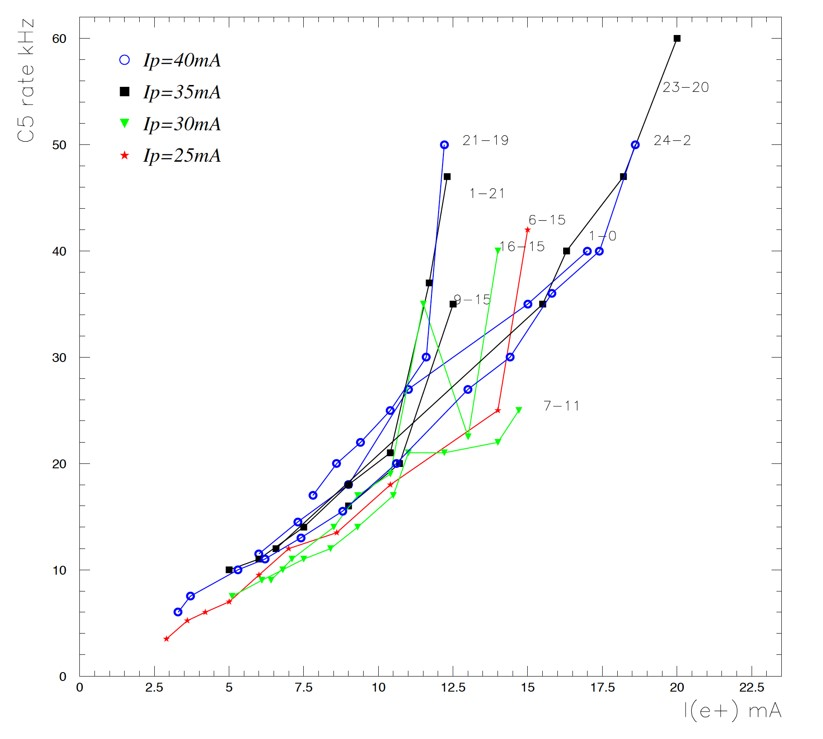
\includegraphics[width=.75\textwidth]{../../img/hera_c5_rate.jpg}
	\caption{C5 rate as a function of HERA \textit{e} beam current for different \textit{p} beam current.  Numeric tags indicate the date and hour of teh beginning of \textit{ep} injection for July 2002.}
	\label{fig:hera3}
\end{figure}


\subsection{Approach}

In order to benchmark simulation tools against HERA background rates, a virtual detector was modeled after the C5 detector and positioned at the same location relative to the IP.  A beam pipe with the same specifications as the original was filled with a hydrogen target of density proportional to the vacuum quality of the corresponding region at HERA.  The orientation of the C5 detector relative to the IP is shown in figure \ref{fig:hera4}.  

\begin{figure}
	\centering
	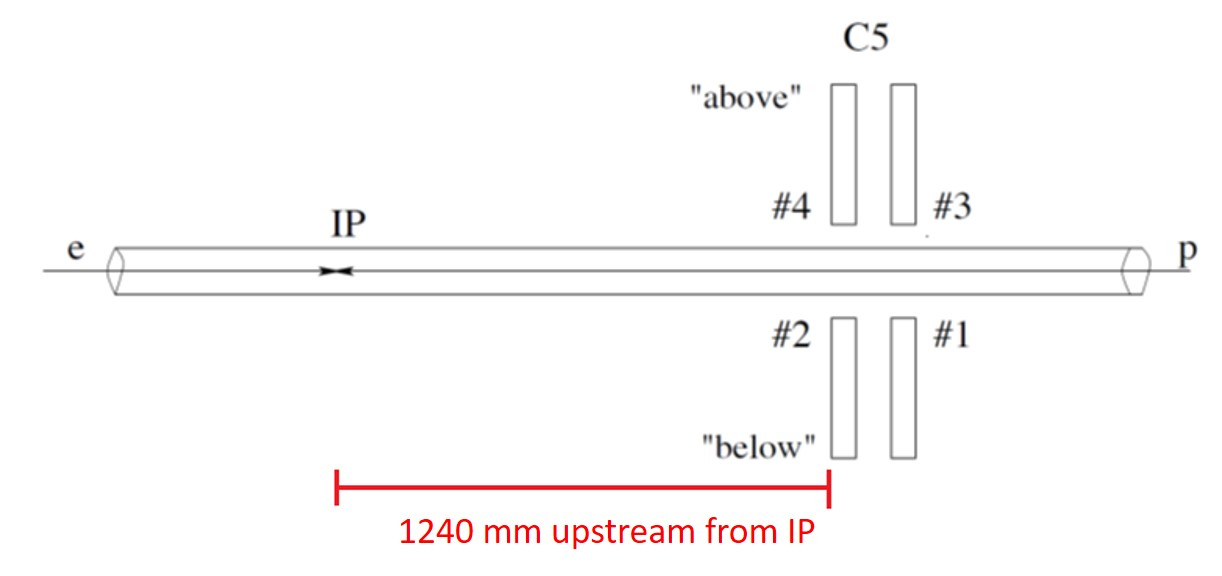
\includegraphics[width=.75\textwidth]{../../img/c5_placement.jpg}
	\caption{C5 detector placement along HERA beamline.}
	\label{fig:hera1}
\end{figure}


Certain parameters were observed or scaled to the study performed.  These are summarized below:
[assumptions/parameters]
\begin{itemize}
	\item HERA-II gate time $\approx$ bunch distance $\approx$ 100ns
	\item Number of proton particles per bunch = $10^{11}$
	\item Proton beam current = 100 mA
	\item Vacuum density in worst region $= 10^{-8}$ mbar.
	\item Poor vacuum region extends $\pm$5m around IP.
	\item In HERA-II, hydrogen gas dominated gas composition.  This simulation assumed 100\% hydrogen gas of density $\rho = 1$ mg*cm$^{-3}$, proportional to $10^{-8}$ mbar.
	\item 

\end{itemize}

To replicate the C5 detector, a two-disc scintillator detector was coded for GEMC and placed 1240 mm upstream of the IP.  Like the actual C5 detector, the virtual detector was copmrised of discs 3 mm thick, separated by 20 mm.  The inner and outer radii were the same: $R_{in} = 3.25/2$ cm and $R_{out} = 20.0/2$ cm.  

\begin{figure}
	\centering
	\begin{minipage}{0.45\textwidth}
		\centering
		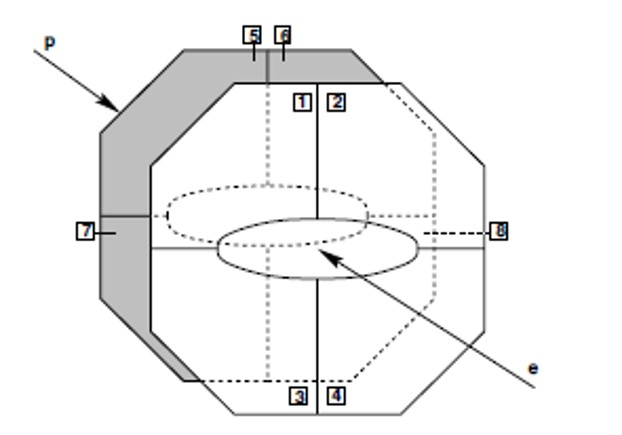
\includegraphics[width=.75\textwidth]{../../img/hera_c5.jpg}
		\caption {Left: Schematic of the actual C5 Time of Flight Detector  }
		
	\end{minipage}\hfill
	\begin{minipage}{0.45\textwidth}
		\centering	\includegraphics[width=.75\textwidth]{../../img/C5_gemc}	
		\caption {Virtual C5 detector rendered in GEMC.}
	\end{minipage}
	
\end{figure}

Likewise, the simple cylindrical beampipe reflected the original beampipe in HERA-II IP.  

- modeled beam pipe with three sections: baseline vacuum "good" vac and "bad vac" 

- positioned particle generator directly in front of bad vac region and fired (beam parameters) towards ip, recorded hits in detector.

- scale hits based on assumptions

- subtract neutral particles that "real" C5 did not see.



\subsection{Results}
- compare rate: achieved comparable rate in our simulation
show: occupancy plot

\subsubsection{vacuum level dependency}
-varied vacuum level

-rate varied as expected

-plot of dependency

\subsubsection{vacuum length dependency}
-varied vacuum length

-rate varied as expected

-plot of dependency

\subsubsection{physics models}

\subsubsection{beam energy independency}


*validity of simulation
\subsection{Conclusion}







%\begin{figure}
%	\centering
%	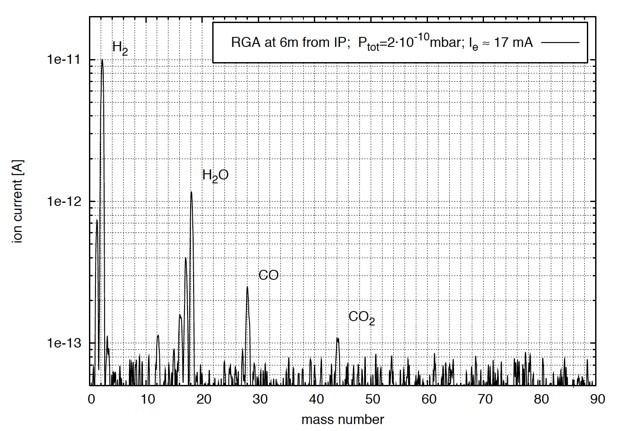
\includegraphics[width=.75\textwidth]{../../img/hera_badvac_comp.jpg}
%	\caption{HERA-II Vacuum pressure distribution in the IR.  The vacuum in the region $\pm$ 5m around the IP deteriorated to $10^{-8}$ mbar, compared to $10^{-10}$ mbar achieved at the pump locations.}
%	\label{fig:hera1}
%\end{figure}

%\begin{figure}
%	\centering
%	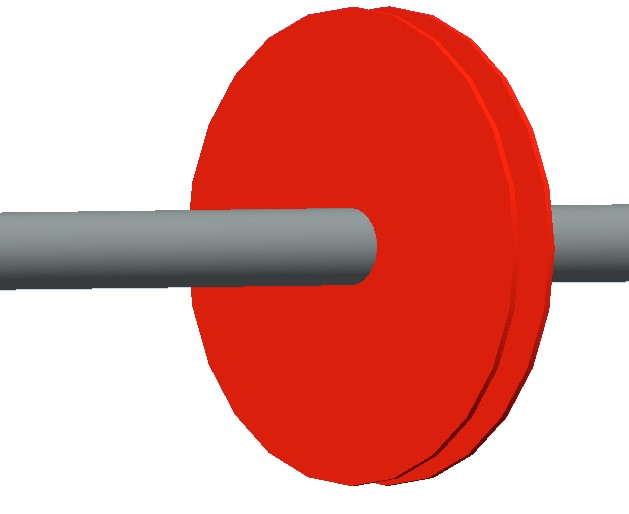
\includegraphics[width=.75\textwidth]{../../img/c5_gemc.jpg}
%	\caption{HERA-II Vacuum pressure distribution in the IR.  The vacuum in the region $\pm$ 5m around the IP deteriorated to $10^{-8}$ mbar, compared to $10^{-10}$ mbar achieved at the pump locations.}
%	\label{fig:hera1}
%\end{figure}

%\begin{figure}
%	\centering
%	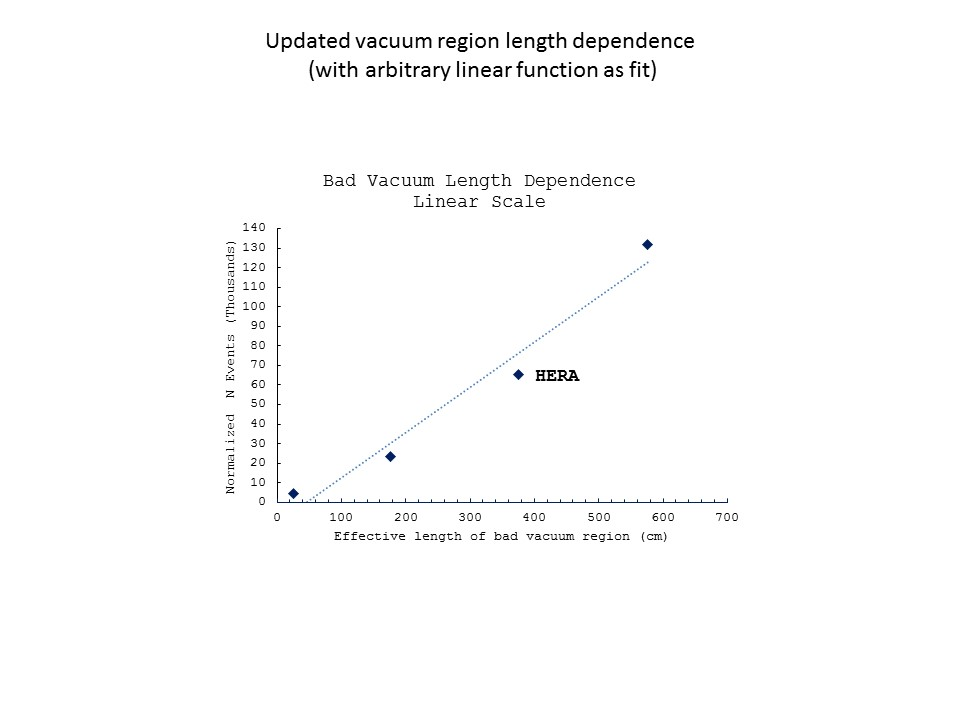
\includegraphics[width=.75\textwidth]{../../img/length_dep_linear.JPG}
%	\caption{HERA-II Vacuum pressure distribution in the IR.  The vacuum in the region $\pm$ 5m around the IP deteriorated to $10^{-8}$ mbar, compared to $10^{-10}$ mbar achieved at the pump locations.}
%	\label{fig:hera1}
%\end{figure}

%\begin{figure}
%	\centering
%	\includegraphics[width=.75\textwidth]{../../img/ length_dep_log.JPG}
%	\caption{HERA-II Vacuum pressure distribution in the IR.  The vacuum in the region $\pm$ 5m around the IP deteriorated to $10^{-8}$ mbar, compared to $10^{-10}$ mbar achieved at the pump locations.}
%	\label{fig:hera1}
%\end{figure}

%\begin{figure}
%	\centering
%	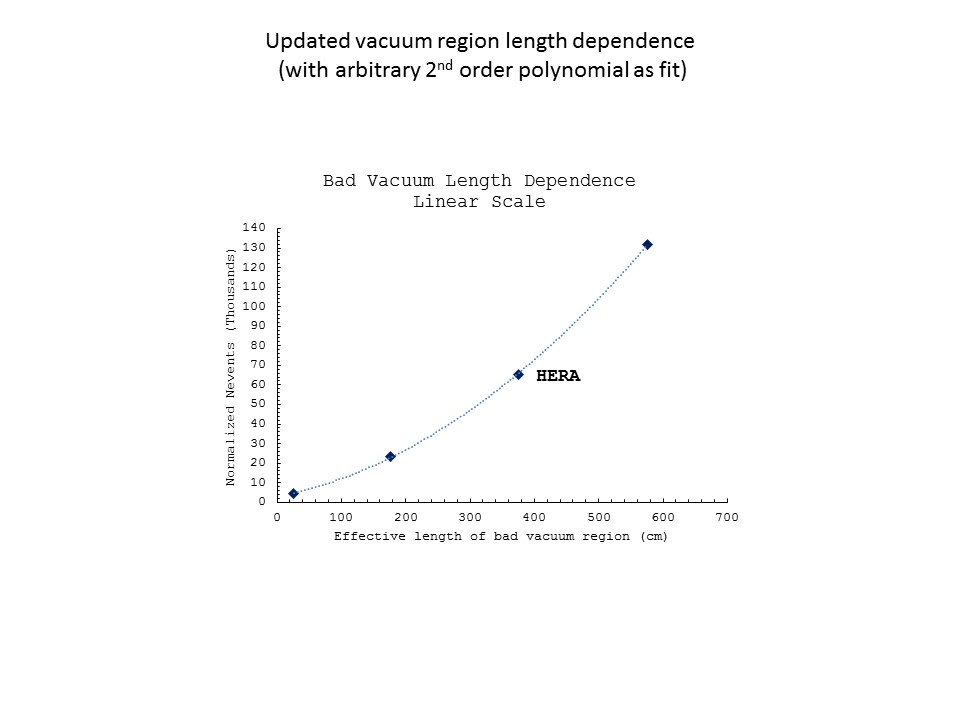
\includegraphics[width=.75\textwidth]{../../img/length_dep_poly.JPG}
%	\caption{HERA-II Vacuum pressure distribution in the IR.  The vacuum in the region $\pm$ 5m around the IP deteriorated to $10^{-8}$ mbar, compared to $10^{-10}$ mbar achieved at the pump locations.}
%	\label{fig:hera1}
%\end{figure}

%\begin{figure}
%	\centering
%	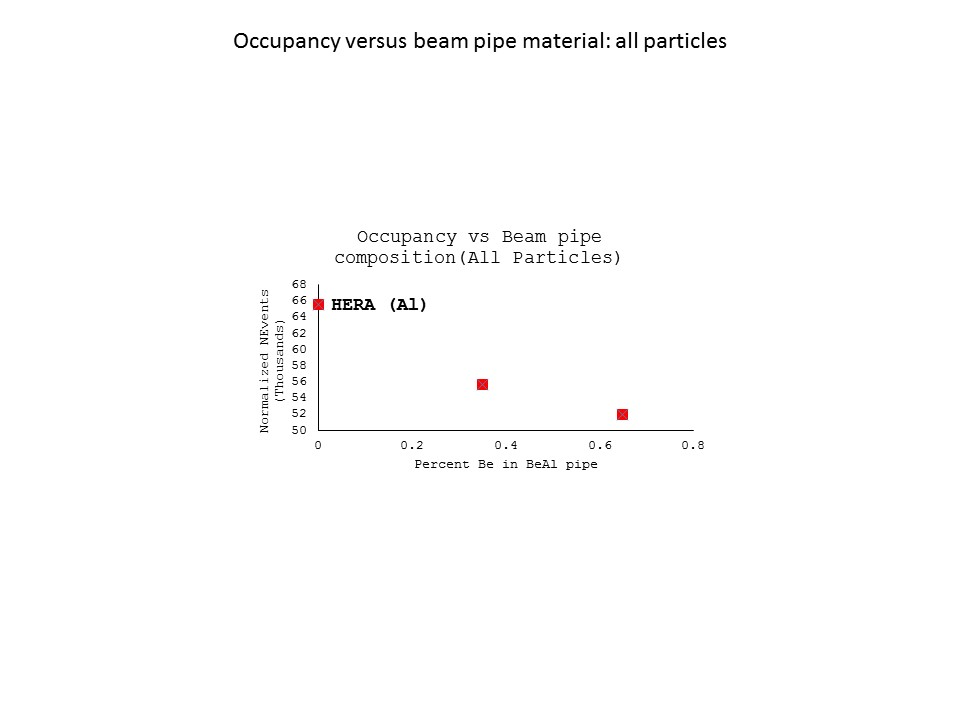
\includegraphics[width=.75\textwidth]{../../img/pipe_comp_all.JPG}
%	\caption{HERA-II Vacuum pressure distribution in the IR.  The vacuum in the region $\pm$ 5m around the IP deteriorated to $10^{-8}$ mbar, compared to $10^{-10}$ mbar achieved at the pump locations.}
%	\label{fig:hera1}
%\end{figure}

%\begin{figure}
%	\centering
%	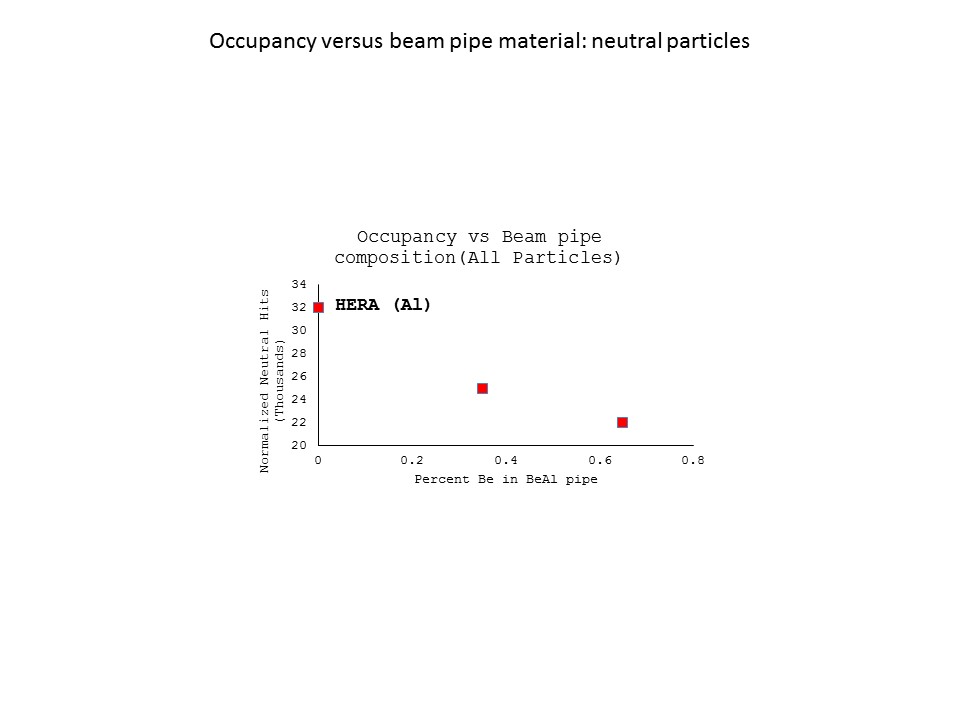
\includegraphics[width=.75\textwidth]{../../img/pipe_comp_neutral.JPG}
%	\caption{HERA-II Vacuum pressure distribution in the IR.  The vacuum in the region $\pm$ 5m around the IP deteriorated to $10^{-8}$ mbar, compared to $10^{-10}$ mbar achieved at the pump locations.}
%	\label{fig:hera1}
%\end{figure}